\begin{figure}[ht!]
    \begin{subfigure}{.5\textwidth}
    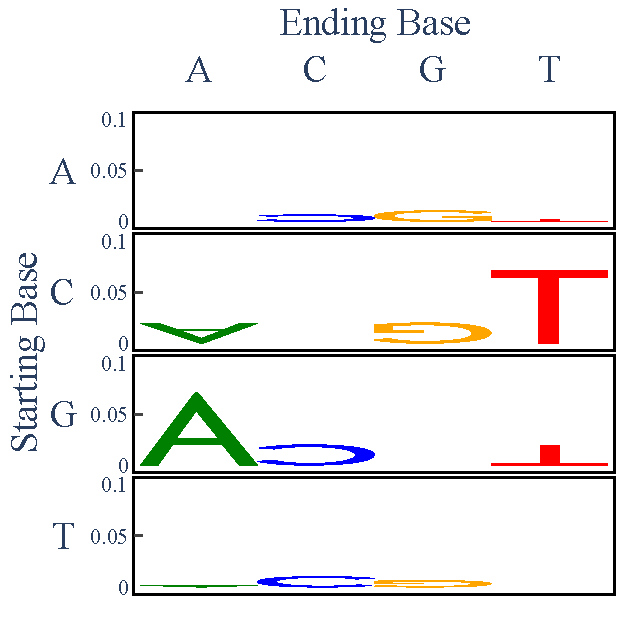
\includegraphics[scale=0.7]{graphics/spectra_Skin-Melanoma.pdf}
    \caption{Skin-Melanoma}
    \label{fig:spectra_skin}
    \end{subfigure}
    ~
    \begin{subfigure}{.5\textwidth}
    
    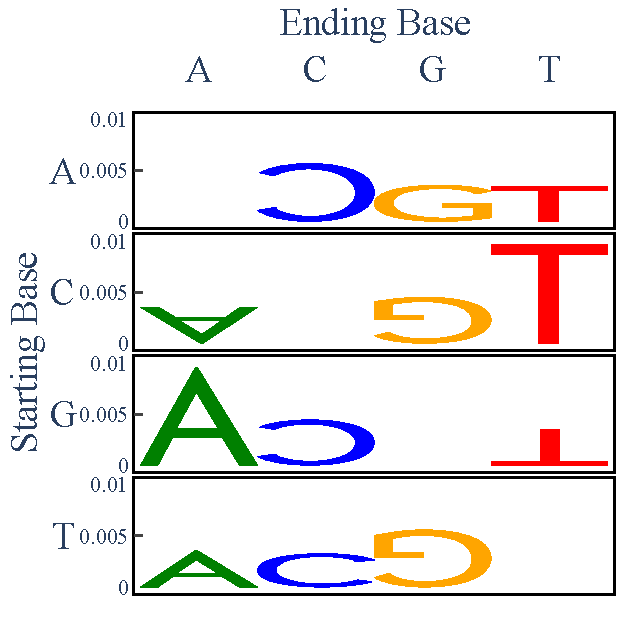
\includegraphics[scale=0.7]{graphics/spectra_Kidney-RCC.pdf}
    \caption{Kidney-RCC}
    \label{fig:spectra_kidney}
    \end{subfigure} \\
    \vspace{0.5cm}
    
    \begin{subfigure}{.5\textwidth}
    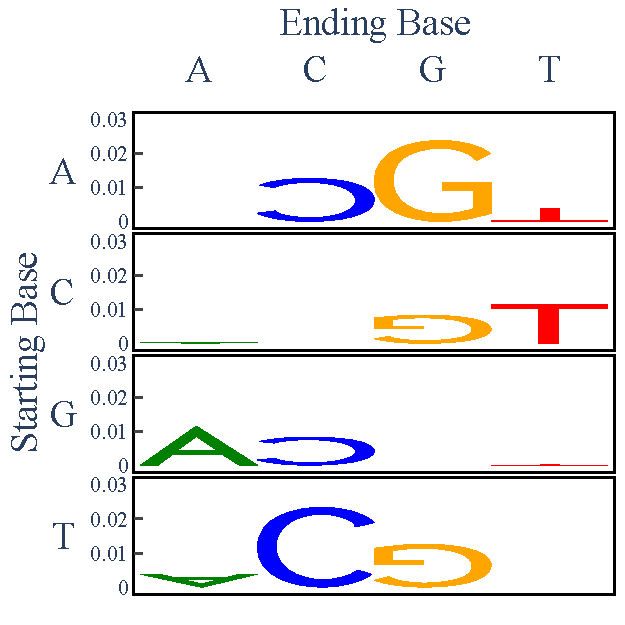
\includegraphics[scale=0.7]{graphics/spectra_Liver-HCC.pdf}
    \caption{Liver-HCC}
    \label{fig:spectra_liver}
    \end{subfigure}
    ~
    \begin{subfigure}{.5\textwidth}
    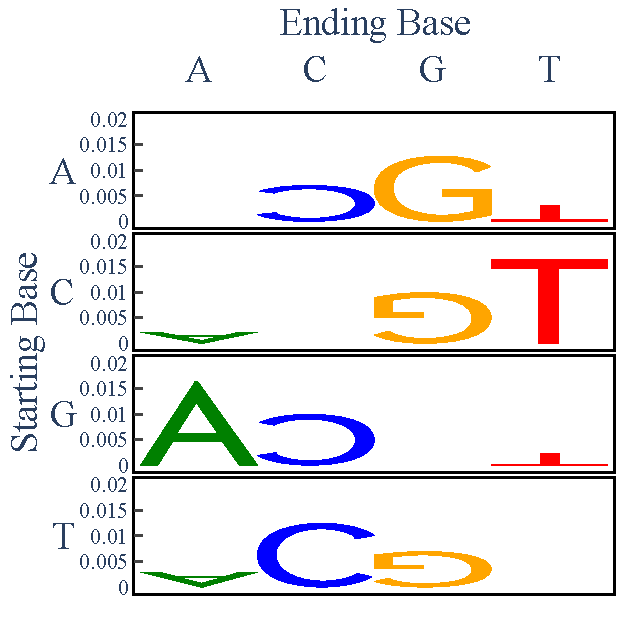
\includegraphics[scale=0.7]{graphics/spectra_Panc-AdenoCA.pdf}
    \caption{Panc-AdenoCA}
    \label{fig:spectra_panc_adenoca}
    \end{subfigure} \\
    \vspace{0.2cm}
\caption{}
    % \caption{\textbf{Base substitutions are a rich source of information}. Here, $RE$'s as a measure of information are shown in mutation logos for (a) Skin-Melanoma (b) Kidney-RCC (c) Liver-HCC (d) Panc-AdenoCA. The other cancers can be found in Figure \ref{fig:apdx_spectra}. For each panel, each row was derived from a pair of GLMs corresponding to a wildtype base. Starting Base is the wildtype base; Ending Base is the product of the substitution. The heights of the letters are $RE$'s for the substituting the Starting Base with the Ending Base. An up-orientation indicates an excess while a down-orientation indicates a deficit of the mutation.}
    \label{fig:spectra}
\end{figure}